\documentclass[11pt]{article}
\setlength{\parindent}{0pt}
\setlength{\parskip}{0.2em} % Adjust '1em' to your preference

\usepackage{geometry}
\geometry{margin=1in}

\usepackage{times}  
\usepackage{helvet}  

\usepackage{amsfonts}
\usepackage{bbm}

\usepackage{graphicx}

\usepackage[utf8]{inputenc}
\usepackage[english]{babel}
\usepackage{hyperref}
\usepackage{natbib}
\bibliographystyle{plainnat}

\usepackage{xcolor}
\newcommand{\todo}[1]{{\color{orange}{TODO: #1}}}
\newcommand{\note}[1]{{\color{blue}{NOTE: #1}}}
\newcommand{\gur}[1]{{\color{teal}{Gur: #1}}}
\newcommand{\yarden}[1]{{\color{magenta}{Yarden: #1}}}


\title{The Effect of Age of Enrollment on the Probability of Graduating from Academic Programs}
\author{Gur Keinan 213635899 \and Yarden Adi 212585848}
\date{October 30, 2024}


\begin{document}

\maketitle

\begin{abstract}
    Many adolescents worldwide have wondered when they should start their journey in higher education. The writers of this project themselves had decided long ago to join the 'Atuda' program, which means starting university at the relatively young age of eighteen. Thus, it is natural to wonder - does the student's age at the start of learning at the university affect the success of the student? An answer to this question can drastically change the landscape of the campuses worldwide and the grades of those studying there. In this Causal Inference project, we aim to explore precisely that. Specifically, we investigate the following causal question: \emph{What is the causal effect of being an adult student (over 21) on the probability of graduating from an academic program?} Throughout this project, we present and explore the data we use to tackle this question and determine its suitability for causal analysis tasks, formally present the methods we use to answer the research question, present and discuss the analysis results, and conclude the project. One can find all of the resources used in the project in this \href{https://github.com/GurKeinan/Causal-Inference-Project-Effect-of-Age-on-Graduating}{GitHub repository}.
\end{abstract}

\gur{changing our question to 'What is the causal effect of enrolling as an adult student (age 21 or older) on the probability of graduating from an academic program within the allotted time?', say somewhere in the paper why we determined the target to be like this}

\textbf{Note on AI Usage:} We did not use generative AI to write this report. We only used ChatGPT, Claude, and Grammarly to revise and correct our writing.

\section{Data Review and Preprocessing}

\gur{Opening sentence.}

\subsection{Data Review}

The data used in our project originated from research done in Portugal by the \href{https://www.ipportalegre.pt/pt/}{Polytechnic Institute of Portalegre} (\gur{Equivalent to college}), as an attempt to provide information to the tutoring team about the risk of students' dropout and failure \citep{data7110146}. Commonly, it is used to build machine learning models for predicting academic performance and dropout (see relevant \href{https://www.kaggle.com/datasets/ankanhore545/dropout-or-academic-success/data}{Kaggle competitions in this subject}).

The data contains information about students' pre-academic background, age, academic performance, social and economic status, and other relevant variables. It consists of 4424 records and 37 variables \todo{number of categorical and numerical}, including the enrollment age. The dataset includes a trinary outcome variable indicating whether a student dropped out, graduated, or is still enrolled in the academic program. 

The data was created by joining 3 primary data sources: 
\begin{enumerate}
    \item CNAES (National Competition for Access to Higher Education) - contains information about students' academic backgrounds, demographics, and course applications at the time of their enrollment in Portuguese higher education institutions.
    \item AMS (Academic Management System) - provides student records data, including demographic information, course enrollments, and academic performance throughout their studies.
    \item PORDATA (Contemporary Portugal Database) - provides macroeconomic data, including unemployment, inflation, and GDP figures.
\end{enumerate}

\gur{Division of the data to classes like in table in the paper}

\todo{Age limitation in Portugal. We can mention and cite that Portugal is said to welcome education in all ages. This statement is commonly used regarding older people, but still.}

\subsection{Data Preprocessing}

\paragraph{Treatment and Target variables} Following our causal question, we introduce a new binary variable - "being over 21". This variable acts as the \emph{treatment variable} in our analysis. We omit the numerical age variable for the rest of the analysis. Additionally, as our question focuses on the probability of graduating from an academic program, we introduce another binary variable - "Graduated from an academic program" rather than the commonly used trinary variable - "graduate/  enrolled/ dropout". This variable is the \emph{target variable} in our analysis. The distributions of the target and treatment variables are visually presented in Figure~\ref{fig:target_and_treatments_histograms}

\begin{figure}
    \centering
    \label{fig:target_and_treatments_histograms}
    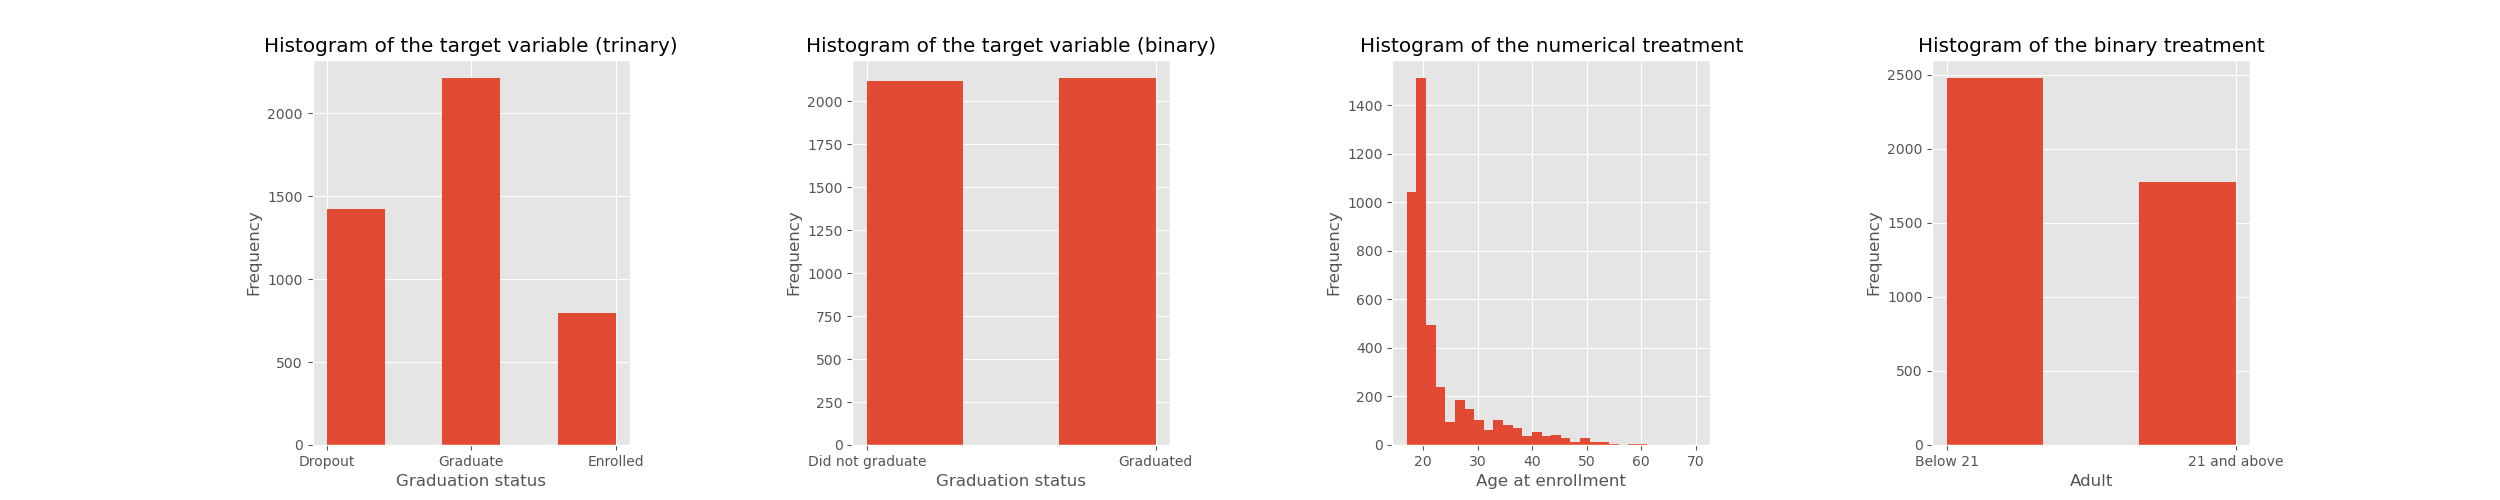
\includegraphics[width = \textwidth]{plots/target_and_treatments_histograms.png}
\end{figure}

\paragraph{Removal of post-treatment variables} The dataset contains multiple variables that had been gathered throughout the students' academic journey, e.g., academic accomplishments, debts, and payment tracking. \yarden{I would write \textbf{despite being informative} instead of \textbf{although informative}} Although informative for machine learning models trying to predict academic dropout, these accomplishments were recorded after the treatment was determined and, therefore, cannot be safely used in the causal inference procedure. We eliminated those variables to maintain the integrity of our results and prevent any post-treatment interference.

\paragraph{Clustering categorical values} The dataset is of impressive complexity and detail, as evident by the categorical variables with over 30 unique values. To perform meaningful analysis, we manually cluster similar categories into one broader category to represent them instead of simply removing the less frequent value. For example, we merged the values 'Armed Forces Professions', 'Armed Forces Officers', and 'Armed Forces Sergeants' into a single 'Armed Forces' value. We performed this procedure on five variables within the data set - the qualifications and occupations of the parents (mother and father) and the student's previous qualifications. 

\paragraph{Pruning categorical outliers} Even after performing the previous step, some variables still contained rare values. After careful consideration and visual inspections, we decided to prune some of the rare values to ease the analysis. The pruning resulted in a sample exclusively consisting of individuals with Portuguese nationality, which may limit the generalizability of this study to a broader population.

\todo{scaling and encoding - I think that it can come later on in the analysis part but don't forget!}


\section{Assumptions for Causal Inference}

In this section, we formally present and discuss four assumptions regarding the nature of our data. Combined, those assumptions guarantee the trustworthiness of an observational causal experiment's results.

\subsection{Stable Unit Treatment Value Assumption (SUTVA)}

The SUTVA assumption consists of two parts. The first one is \emph{no interference}, which requires that the potential outcomes of each unit are not affected by the treatment assignment of any other unit; the second is \emph{no hidden variations of treatment}, which forbids the existence of different forms or versions of each treatment level, which lead to different potential outcomes.

In our experiment, the treatment variable, 'enrolling as an adult student (over 21)' \gur{is it?}, is well-defined and has only two versions. Hence, the second part of the assumption safely holds. The assumption's first part holds if we presume one student's adulthood does not affect the probability of his fellow student graduating from the program, which is controversial. There are several aspects in which the varied spectrum of ages on the campus might affect the students' success. Such elements include but are not limited to 1) peer effects - encountering different perspectives and learning methods (that can be related to one's age) might affect one's abilities; and 2) In competitive programs, students' success may be directly affected by their peers' accomplishments. Therefore, if age is indeed related to one's academic achievements, one student's age can indeed affect another's success.

\subsection{Consistency}

The Consistency assumption states that an individual's potential outcome under his or her observed exposure history is the outcome that will actually be observed for that person. Put formally, for a unit that receives treatment $T$, we observe the corresponding potential outcome $Y = TY_1 + (1-T)Y_0$. This assumption can be violated when the individual's history is misreported. Since our data was extracted from credible and regulated sources and processed using careful and documented manipulations, we believe that the Consistency assumption likely holds in our study. 

\gur{elaborate more? Data Source Reliability, Clear Treatment Definition, Outcome Measurement, Data Processing Transparency, Stable Treatment}


\subsection{Ignorability - No Unmeasured Confounders}

The Ignorability assumption states that the treatment assignment $T$ is independent of the potential outcomes $Y_0, Y_1$ given the observed covariates $X$, i.e., $Y_0, Y_1 \perp T \ | \ X$. 

\gur{'Unverifiable assumption.' https://www.ncbi.nlm.nih.gov/pmc/articles/PMC10666970/}

\gur{'We close with a reminder to readers of the optimistic view of the complexity of data and how the correlation between observed variables and unmeasured ones can reduce any bias associated with unmeasured information.' https://www.ncbi.nlm.nih.gov/pmc/articles/PMC10666970/}

\subsection{Common Support (Overlap)}

The Common Support assumption states that each unit has a non-zero probability of receiving each treatment level, i.e., $\forall x \in X, P(T=1|X=x) > 0$ and $P(T=0|X=x) > 0$.

We empirically validate this assumption using propensity scores. We trained a logistic regression model to predict the treatment assignment based on the covariates, and used the predicted probabilities as the propensity scores. We then plotted the propensity scores of the treated and control groups to ensure that there is a significant overlap between the two groups. The results are presented in Figure \ref{fig:common_support}. The lowest predicted propensity score of the treated group is $0.0209$, and the control group's is $0.009$. Therefore, we conclude that the common support assumption holds in our data.

\begin{figure}
    \centering
    \caption{Common support of the propensity scores}
    \label{fig:common_support}
    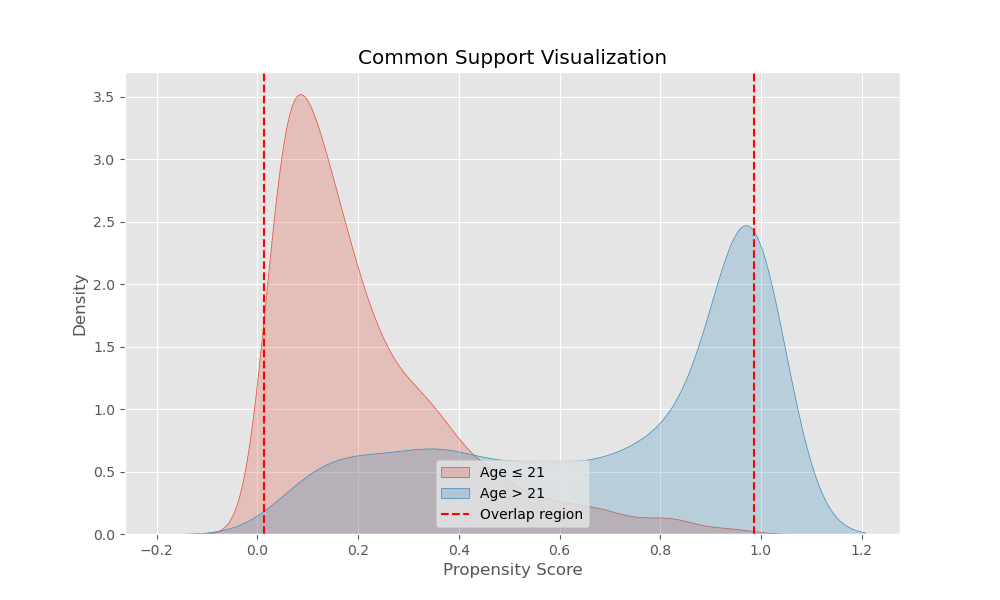
\includegraphics[width = 0.8\textwidth]{plots/common_support.png}
\end{figure}



\section{Causal Analysis Methodology}

After validating the assumptions for causal inference, we describe the methodology used to perform the causal analysis. We present the relevant measures of causal effects and the methods we use to estimate them.

\subsection{Measures}

To quantify the causal effect of the treatment on the outcome, one usually tries to estimate the Average Treatment Effect (ATE). However, in some cases, estimating the Average Treatment Effect on the Treated (ATT) or the Average Treatment Effect on the Control (ATC) is more informative. We formally present those measures below.

\paragraph{Average Treatment Effect (ATE)} Defined as the difference between the expected outcome under treatment and the expected outcome under control. Formally, it is defined as $ATE = E[Y_1 - Y_0]$.

\paragraph{Average Treatment Effect on the Treated (ATT)} Defined as the difference between the expected outcome under treatment and the expected outcome under control, but only for the treated units. Formally, it is defined as $ATT = E[Y_1 - Y_0 | T = 1]$. 

\paragraph{Average Treatment Effect on the Control (ATC)} Defined as the difference between the expected outcome under treatment and the expected outcome under control, but only for the control units. Formally, it is defined as $ATC = E[Y_1 - Y_0 | T = 0]$. 

Each of the three measures provides a different perspective on the causal effect of the treatment. The ATE measures the average effect of the treatment on the entire population. In contrast, the ATT and ATC measures provide insights into the effect of the treatment on the treated and control units, respectively. The ATT and ATC measures are notably helpful when the treatment assignment is not controlled (not random), as in observational studies.

\paragraph{Bootstrap-based confidence intervals} \todo{Complete this.}

\subsection{Methods}

\gur{Covariate adjustment, IPW, propensity score matching, doubly robust}

\gur{Estimate ATE, ATT, and derive ATC through the mathematical relation}

\gur{For Covariate adjustment, calculate ATE as usual, calculate ATT by only iterating over the treated group and ATC by only iterating over the control}

\gur{For IPW, use TA5 and derive ATC through the mathematical relation between ATE, ATT and ATC}

\gur{For propensity score matching, calculate ATT and ATC by matching treated to control and control to treated, respectively, and derive ATE through the mathematical relation between ATE, ATT and ATC}

\gur{For the doubly robust, use the paper I put in the references and cite it for all three.}

The fundamental problem of causal inference is that directly observing causal effects is impossible. It is impossible to observe both potential outcomes of the units and compute the impact of the treatment. In the remainder of this section, we present the estimation methods we used in our analysis, explain how they are trying to handle the mentioned problem, present the assumptions each requires for truthfully estimating the causal effects, and detail the implementation of each method.


\subsection{Covariate Adjustment}

Covariate adjustment methods use statistical models to regress the missing potential outcomes based on the observed covariates and the treatment. The regressed values are then used to estimate the average treatment effects.

There are different covariate adjustment methods, where the separation between them is usually found in if and how to separate the treatment variable from the covariates while regressing the missing potential outcomes and how to use the regressed values for the average effect estimation. We used the methods \emph{S-Learner} and \emph{T-Learner} for our analysis.

\gur{Theoretical guarantees?}

\paragraph{S-Learner} Addresses the treatment variable $T$ as one of the covariates. First, one must learn a statistical model for predicting the conditional average treatment effect (CATE) as a function of the covariates $X$ and the treatment $T$ - $\hat{\mu}(X, T) = \hat{\mathbb{E}}[Y^{obs} | X, T]$. Any ML method can be used for this purpose, but importantly, the whole population is used to learn the model. Then, use the learned model to estimate the average treatment effects as follows:

\begin{itemize}
    \item \textit{ATE:} Average the predicated causal effect on all of the population:
    \[
    \widehat{ATE} = \frac{1}{n} \sum_{i=1}^{n} \hat{\mu}(x_i, 1) - \hat{\mu}(x_i, 0)
    \]
    \item \textit{ATT:} Average the predicted causal effect on the treatment group:
    \[
    \widehat{ATT} = \frac{1}{\sum_{i=1}^{n} t_i} \sum \sum_{i=1}^{n} t_i \left[ \hat{\mu}(x_i, 1) - \hat{\mu}(x_i, 0) \right] 
    \]
    \item \textit{ATC:} Average the predicted causal effect on the control group:
    \[
    \widehat{ATC} = \frac{1}{\sum_{i=1}^{n} 1 - t_i} \sum \sum_{i=1}^{n} (1 - t_i) \left[ \hat{\mu}(x_i, 1) - \hat{\mu}(x_i, 0) \right]
    \]
\end{itemize}

\paragraph{T-Learner} Uses observations in the treatment group to estimate the response under control, $\hat\mu_1(x) = \hat{\mathbb{E}}[Y^{obs} | X, 1]$. Similarly, use observations in the control group to estimate the response under treatment, $\hat\mu_0(x) = \hat{\mathbb{E}}[Y^{obs} | X, 0]$. Any machine learning method can be used to get these estimates. Calculating the average effects continues similarly to the S-Learner with $\hat \mu (X_i, T)$ replaced with $\hat \mu_T(x)$.

\paragraph{Implementation Details} \todo{}

\gur{Add RMSE comparison between different regression models, argue that we do that because the guarantees only work if the regression model is exact.}

\subsection{Propensity-Based Methods}

One of the problems with covariate adjustment methods is the sensitivity to model simplification and the sparsity of the covariates when handling high-dimensional data \citep{zhao2020propensity}. The propensity score methods of Rosenbaum and Rubin (RR) aim to address the fundamental problem by adjusting for the propensity score rather than potentially high-dimensional covariates. RR demonstrated that under the assumption of no unmeasured confounding, this is enough for unbiased estimation of causal effects and such estimation can be accomplished using simple non-parametric methods.

\paragraph{Inverse Probability Weighting} Relies on building a logistic regression model to estimate the probability of the exposure observed (i.e., the propensity score) for a particular individual and using the predicted probability as a weight in subsequent analyses. Our analysis uses the Horvitz–Thompson estimator \citep{horvitz1952generalization}. Intuitively, it estimates the target variable's mean in the treatment and control groups by weighting the observations based on their "membership". One must first train a logistic regression model for predicting the propensity score $\hat e(x) = \hat P(T=1 | X=x)$. Then, use it to weigh each of the samples in the following way to receive each of the average effects:

\begin{itemize}
    \item \textit{ATE:} \todo{}
    \[
    \widehat{ATE} = \frac{1}{n}\sum_{i=1}^N \frac{t_i y_i}{e(x)} - \frac{1}{n}\sum_{i=1}^N \frac{(1-t_i)y_i}{1-e(x)}
    \]

    \item \textit{ATT:} \todo{}
    \[
    \widehat{ATT} = \frac{\sum_{i=1}^N t_i y_i}{\sum_{i=1}^N T_i} - \frac{\sum_{i=1}^N (1-t_i)y_i \cdot \frac{e(x_i)}{1-e(x_i)}}{\sum_{i=1}^N (1-t_i) \cdot \frac{e(x_i)}{1-e(x_i)}}
    \]
    \item \textit{ATC:} \todo{}
    \[
    \widehat{ATC} = \frac{\sum_{i=1}^N t_iy_i * \frac{1-e(x_i)}{e(x_i)}}{\sum_{i=1}^N t_i * \frac{1-e(x_i)}{e(x_i)}} - \frac{\sum_{i=1}^N (1-t_i)y_i}{\sum_{i=1}^N (1-T_i)}
    \]
\end{itemize}


\paragraph{Propensity Score Matching} Propensity Score Matching is a method that groups treated and control units with similar propensity scores. This method is often thought of as attempting to replicate a randomized controlled experiment, as it tries to create (in some sense) a similar balance in observed variables between the treatment and control groups. After matching the units, the causal effect of the treatment can be estimated by averaging the differences in outcomes between the matched treated and control units in each group.

\paragraph{Implementation Details} \todo{}

\gur{Add ROC curve of several binary classification models, argue that we do that because the guarantees only work if the propensity is exact.}


\subsection{Doubly-Robust Method}


Doubly Robust Estimation is a method that fortuitously combines outcome regression and propensity score weighting methods to estimate the causal effect of the treatment. Formally, given the observed outcome $Y$, the treatment assignment $T$, and the covariates $X$, the Doubly Robust Estimator is defined as:

\gur{Add the formula here.}

The Doubly Robust Estimator is consistent (not biased) if either the outcome regression model or the propensity score model is correctly specified, making it a robust method for estimating causal effects.

\paragraph{Implementation Details} \todo{Details about the implementation of the Doubly Robust Estimator.}







\section{Results}

\begin{itemize}
    \item One graph to compare all of the results from the methods (box plots).
    \item Discussion.
    \item Analyze correlation / dominant features.
\end{itemize}

\section{Discussion}

\begin{itemize}
    \item Conclusions
    \item Possible weaknesses.
    \item Avenues for future work.
\end{itemize}

\bibliography{references.bib}

\appendix

\end{document}